%-----------------------------------------------
% Template para criação de resumos de projectos/dissertação
% jlopes AT fe.up.pt,   Fri Jul  3 11:08:59 2009
%-----------------------------------------------

\documentclass[9pt,a4paper]{extarticle}

%% English version: comment first, uncomment second
%\usepackage[portuguese]{babel}  % Portuguese
\usepackage[english]{babel}     % English
\usepackage{graphicx}           % images .png or .pdf w/ pdflatex OR .eps w/ latex
\usepackage{times}              % use Times type-1 fonts
\usepackage[utf8]{inputenc}     % 8 bits using UTF-8
\usepackage{url}                % URLs
\usepackage{multicol}           % twocolumn, etc
\usepackage{float}              % improve figures & tables floating
\usepackage[tableposition=top]{caption} % captions
%% English version: comment first (maybe)
%\usepackage{indentfirst}        % portuguese standard for paragraphs
%\usepackage{parskip}

%% page layout
\usepackage[a4paper,margin=30mm,noheadfoot]{geometry}

%% space between columns
\columnsep 12mm

%% headers & footers
\pagestyle{empty}

%% figure & table caption
\captionsetup{figurename=Fig.,tablename=Tab.,labelsep=endash,font=bf,skip=.5\baselineskip}

%% heading
\makeatletter
\renewcommand*{\@seccntformat}[1]{%
  \csname the#1\endcsname.\quad
}
\makeatother

%% avoid widows and orphans
\clubpenalty=300
\widowpenalty=300

\begin{document}

\title{\vspace*{-8mm}\textbf{\textsc{Exploring Visual Programming Concepts\\for Probabilistic Programming}}}
\author{\emph{Gabriel Cardoso Candal}\\[2mm]
\small{Dissertation done under the supervision of \emph{Prof.\ Hugo Sereno Ferreira}}}
\date{}
\maketitle
%no page number
\thispagestyle{empty}

\vspace*{-4mm}\noindent\rule{\textwidth}{0.4pt}\vspace*{4mm}

\begin{multicols}{2}

\section{Motivation}

There is, among several domains with interesting and relevant problems to solve (computer vision,
cryptography, biology, fraud detection, recommender systems, ...) \cite{intml}, the recurring
necessity to be able to make decisions in the face of uncertainty using machine
learning (ML) methods.
One of the ML approaches that can me used to tacke the problem is to build a
probabilistic model through the use of a probabilistic programming language (PPL),
which lets you write your model as a program and have off-the-shelf inference \cite{Prekopa2003}.
Despite PPLs’ power and flexibility, it's difficult for their target audience
(data scientists, statisticians, mathematicians, ...) to adapt to the textual
interface these languages provide, which lack the graphical intuition provided
by other tools they are accustomed to. We believe this negatively affects
productivity and slows down the adoption of PPLs \cite{darpa}.

\section{Goals}

We aim to overcome
the difficulties in learning a new language, either for inexperienced developers or seasoned
ones, such as learning yet another syntax or getting accustomed to the language’s idioms. It is
known that typical languages are difficult to learn and use \cite{Lewis1987} and that there are advantages in
providing a language with a visual interface \cite{dfbeg}.

The goal of this dissertation was to develop a Visual Programming (VP) language with
probabilistic programming capabilities. The target audience is programmers and data scientists
with background knowledge in statistics which aren’t still comfortable with full blown PPLs, but
wish to educate themselves on the topic so they can eventually leverage the power of this novel
machine learning approach.

\section{Work description}

During this dissertation we have developed a Visual Programming Environment (VPE),
a tool which allows the user to design its model graphically and then either
execute it or translate it into code (we chose to generate Infer.NET code,
a probabilistic programming library from Microsoft that is compatible with CLR
languages such as C\#, F\# or IronPython).

By doing so we have provided a tool which can be used to make usability research
on. For instances, it allows future studies where it could be empirically assessed if the hypothesis that people
with knowledge in statistics can learn to use a PPL faster using VP
rather than the traditional textual form. We have also shown that it is possible
to represent a probabilistic program in a graphical manner by representing several
probabilistic programs with a variety of features using our tool, one of them being
represented in Fig. \ref{fig:first}.

\begin{figure}[H]
\centerline{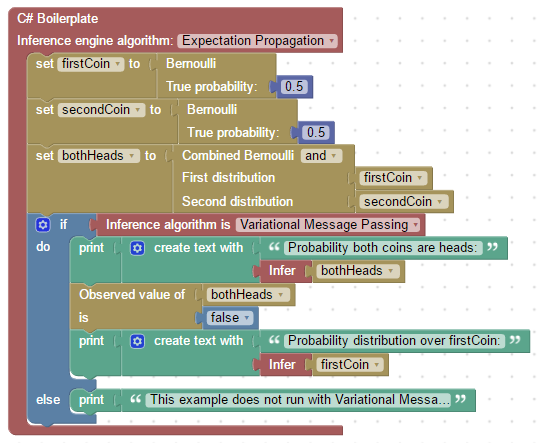
\includegraphics[scale=.6]{firstExample.png}}
\caption{Example of a probabilistic model in our VPE.}
\label{fig:first}
\end{figure}

During this process, we had to make choices regarding both the paradigms and the
technologies in which we would base our VPE on, and we
describe some of them below. In addition to detailing those choices, we are
using the remainder of this section to elicit some VP concepts
we find useful to have in a VP language for probabilistic programming.

\subsection{Purely Visual vs Environment}

The difference between a VPE and a purely visual language is that, while a purely visual language is a language \textit{per se}
(meaning that it there is a direct mapping between graphics and execution), VPEs offer a middle
ground between regular textual languages and purely visual languages: they provide a graphical interface that can
be used to generate code for a target language \cite{Burnett1999}. These two
concepts are often refered in the literature as if they were mutually exclusive,
but we included both of them: we have a VPE that can execute code, so that the
user can get results sooner (does not require code to be copied to a separate
environment) so that the visual feedback can be as immediate as possible, which
is something essential in VP \cite{Shu1988}.

\subsection{Dataflow vs Blockly}

When choosing how to visually represent a model visually, we had to make a choice
between these two alternatives. While visual dataflow programming is used in
successful commercial applications such as RapidMiner and Blender, Blockly-like
representations are most seen in educational tools such as MIT's Scratchy.

Due to the nature of our target audience, we thought that it would be suitable
for our tool to offer a representation that could generate more human-like code,
so that users could look use the tool as a safety net to generate code as if they
were the ones writing it, until they are proficient enough that they won't need
the VPE. Because of this, we decided to use a Blockly-like representation.

\subsection{Visual Programming Concepts}

There are a set of visual programming concepts that seem essential to include
so that the user can be faster and make fewer mistakes when developing using
any VP tool, such as:

\begin{itemize}
  \item Comments
  \item Duplicate blocks
  \item Search blocks by name
  \item Use of icons and colors to convey meaning
  \item Get help (be able get details about a block's functionality)
  \item Serialization (save and load programs while also being able to share them)
  \item Zoom, block collapsing and compression (minize used space when details are not
  important)
  \item Minimap (have a bird's eye view over the program and be able to
  focus a specific area)
\end{itemize}

\subsection{Type safety}

Because we see a VPE based on a Blockly-like representation to be best suited for
educational purposes, it is of the utmost importance to have type safety. This
means that, besides not being able to represent a program with synactic errors,
it is also impossible to make type mistakes (such as trying to use a boolean value
to specify the mean of a gaussian distribution).
This is done in a natural manner: like in a puzzle, blocks that violate type
safety can't be connected. This is better than waiting for a compiler or run-time
error, since the mistake is caught sooner and the visual feedback is as fast as
possible.

\subsection{Function Blocks}

A visual programming concept that deserves a reference of its own are function blocks.
This means empowering the user to create blocks made of blocks, which a concept
analogous to functions or macros in programming. Providing such a feature helps
transforming a VP language in one of an higher level, since users can iterate
on the construction of these blocks and abstract complexity.

\section{Conclusions}\label{sec:conclui}

It is our belief that the graphical representation is clearer than its textual counterpart, mainly
because parameters are named and due to the use of colors.

The main reason to use a VPE rather than the original textual representation is because of the
safety net it provides and which prevents the user from making either syntax or type errors.
Because of this, we believe this kind of visual programming environment can be useful to
help data scientists who are inexperienced programmers take the first steps in using a PPL.

However, if we don’t look at the VPE as an educational tool but rather as something that
won’t be transitional, we think that productivity-wise it falls short when compared to tools such as
RapidMiner, Excel or even textual representations. The main rationale behind this is that, because
we chose to adopt a Blockly representation, the resulting VPE is not a completely visual language
since it violates concreteness and does not fully encapsulate textual programming concepts (such
as variable declarations). If there was someone considering to develop a VPL to be used as a
permanent substitute to the textual form of PPLs, we believe he should explore a dataflow representation,
which is at an higher-level of abstraction than Blockly and has been used in successful
applications both in industry and academia.

%%English version: comment first, uncomment second
%\bibliographystyle{unsrt-pt}  % numeric, unsorted refs
\bibliographystyle{unsrt}  % numeric, unsorted refs
\bibliography{refs}

\end{multicols}

\end{document}
